\documentclass{article}
\usepackage{amsmath, amsfonts, amssymb, amsthm, stmaryrd}
\usepackage{enumitem}
\usepackage{hyperref}
\usepackage{bbm}
\usepackage{algorithm2e}

\usepackage[verbose=true,letterpaper]{geometry}
\newgeometry{
  textheight=9.5in,
  textwidth=6.5in,
  top=0.5in,
  headheight=12pt,
  headsep=25pt,
  footskip=30pt
}
\setlength{\parskip}{0.5em} % blank lines between paragraphs
\usepackage{tikz}
\usepackage{pgfplots}

%%%%%% Commands and theorems
\theoremstyle{plain}
\newtheorem{Theorem}{Theorem}
\newtheorem{Proposition}{Proposition}
\newtheorem{Corollary}{Corollary}
\newtheorem{Lemma}{Lemma}

\theoremstyle{remark}
\newtheorem{Definition}{Definition}
\newtheorem{Assumption}{Assumption}

\renewcommand{\P}{\mathbb{P}}
\newcommand{\E}{\mathbb{E}}
\newcommand{\R}{\mathbb{R}}
\newcommand{\N}{\mathbb{N}}

\newcommand{\sign}{\text{sign}}
\newcommand{\1}{\mathbbm{1}}

\newcommand{\argmin}{\arg\min}

\usepackage{color}
\usepackage{array}
\newcolumntype{L}[1]{>{\raggedright\let\newline\\\arraybackslash\hspace{0pt}}m{#1}}
\usepackage{todonotes}
\newcommand{\todoT}[1]{\todo[inline,color=blue!40]{{\textbf{T:}~}#1}}

\usepackage{enumitem}

% Have descriptions with italic and bullets:
\setlist[description]{font=\normalfont\itshape\textbullet\space}
% To include the section number in the equation numbering:
\numberwithin{equation}{section}

\title{Adaptive stopping in Monte-Carlo evaluation for Deep RL}
\date{}
\begin{document}
\maketitle
\section{Description of the problem}
In Reinforcement Learning, we often use Monte-Carlo methods to evaluate the performances of an algorithm. In particular, if we denote $e(A)$ some evaluation of algorithm $A$, the global score of an algorithm by
$$S(A)=\frac{1}{N}\sum_{i=1}^N e_i(A) $$
where $e_1(A), \dots,e_N(A)$ are the evaluation of the algorithm $A$ on $N$ different seeds (i.e. $e_1(A),\dots,e_N(A)$ are supposed i.i.d).

\subsection{Goal and requirements for the algorithm}

The goal of this article is, given two agents $A_1$ and $A_2$, to evaluate how high $N$ must be to be certain that either $\E[e_1(A_1)]=\E[e_2(A_2)]$ or $\E[e_1(A_1)]\neq \E[e_2(A_2)]$, i.e. do the two algorithms perform similarly or is one better than the other ? This is a trade-off between computational time and the need to assess correctly the scores of $A_1$ and $A_2$. The main properties that we want for our algorithm are as follows:

\begin{description}
\item[Multiprocessing] The algorithm should be able to treat batch of datas.
\item[Non-Parametric] The algorithm should be non-parametric.
\item[Fixed Budget] The algorithm should have a fixed maximum number of iterations used.
\item[Sample efficient] The algorithm should stop as soon as possible in practice.
\end{description}

One algorithm that verifies all the properties listed above is a group sequential permutation test that we will describe in this article.

\subsection{Alternative approaches}

\paragraph{Fully Sequential testing}
In the sequential testing setting, the data are handled one after the other, there is no batch of data. This is not adapted to our problem because in practice, one is often capable of training several agents in parallel, hence the evaluations are received by batch.

\paragraph{SPR/GLR test}
A particular class of sequential test often used are the Sequential Probability Ratio test and the Generalized Likelihood Ratio test. Both of these tests could be generalized to a group-sequential context but they both depend strongly on a parametric model for the data. However, the reward distribution of RL algorithms is often heavy-tail and multi-modal and as a consequence it is difficult to use a parametric model to represent all of them efficiently and simultaneously for several agents, each with a different reward distribution. Moreover, because we want to deal with small sample-sizes, the asymptotic of the central limit theorem is not adapted.

\paragraph{Bandits (Best arm identification or Ranking)} Our objective is close to the objective of ranking bandits algorithms. However compared to bandits we want to at the same time \textit{minimize the stopping time} (similar to fixed-confidence setting) of the algorithm and have a \textit{fixed maximum budget} (similar to fixed-budget setting). In our algorithm we allow for a type I error of $\alpha \in (0,1)$, which is very similar to the fixed confidence setting while still having a fixed budget. Then, compared to the fixed budget setting we allow a larger error rate and as a consequence we are more sample efficient than bandits algorithms.



\section{Adaptive stopping using Group Sequential Testing}
\subsection{Group sequential testing}
\todoT{Explain why must be careful when doing GIT and that we can't just do several tests. Maybe also motivate using the confidence interval approach from NIPS article.}

To choose $N$ adaptively, we propose to use group sequential testing (GST). GST are used in particular in clinical trials in which case an early stopping is desirable when comparing two drugs. We choose to use GST in particular and not sequential testing because the data are often naturally grouped due to the parallelization of the computation.

GST often suppose strong models on the data, in particular it is often supposed that the data are i.i.d. from a Gaussian distribution. This assumption is often not verified in the case of $e_i(A)$ being evaluations from a RL algorithm. In particular, the distribution of $e_i(A)$ often presents several modes and it can sometimes contain outliers.

\todoT{Explain why several modes and give examples of distributions of DeepRL algos on classical environments. Ref https://arxiv.org/pdf/1806.08295.pdf on this also.}

The presence of several modes in the distributions of the evaluations and the difficulty to make any distributional assumption justify a non-parametric approach of the problem, but to further justify this approach we did a study of the effect of model misspecification on simulated data when using Gaussian GST algorithm.


For now, we suppose that $e(A)$ is a continuous random variable, in particular $\P(e_i(A)=e_j(A))=0$ for any $i \neq j$.

\subsection{Algorithm}

\subsection{High level description of the algorithm}
We use the following algorithm.

\begin{algorithm}[h]
\SetAlgoLined
\SetKwInput{KwParameter}{Parameters}
\KwParameter{Agents $A_1,A_2$, environment $\mathcal{E}$, number of blocks $K \in \N^*$, size of a block $n$, level of the test $\alpha\in (0,1)$.}
Define $2nK$ different seeds $s_{1,1},\dots,s_{1,n},s_{2,1},\dots,s_{2,n}$.\\
\For{$k=1,\dots,K$}{
\For{$i=1,2$}{
Train agent $A_i$ on environment $\mathcal{E}$ with the seeds $s_{i,kn},\dots,s_{i,(k+1)n}$.\\
Collect evaluations $e_{kn}(A_i),\dots,e_{(k+1)n}(A_i)$.\\
Compute $S_t(A_i)=\frac{1}{nk}\sum_{j=1}^{nk}e_{j}(A_i)$.\\
}
Compute the boundary $B_k$ of the current block using the permutation distribution of the difference of means of $e_{1}(A_1),\dots,e_{(k+1)n}(A_1),e_{1}(A_2),\dots,e_{(k+1)n}(A_2)$.\\
\If{$|S_t(A_1)-S_t(A_2)| \ge B_k$}{
Reject the equality of the agents' evaluation, break the loop and returns the answer
}
\Else{
If $k=K$ then accept the equality of the agents' evaluation, otherwise continue.
}
}
If the test was never rejected, return accept. Else return reject.
\caption{Adaptive Stopping.}\label{alg:adastop_2}
\end{algorithm}
\todoT{Write a small algorithm to explain how to compute $B_k$ using Equation~\eqref{eq:def_Bk}, with an alternative version for the random permutation version.}

An illustration of the group sequential test is given in figure~\ref{fig:gst}. The boundary in blue is computed sequentially to have a final level $1-\alpha$ for the test, the red points are the observed values of the test statistic (denoted $w_i$). The algorithm stops at the third iteration $k=3$ because the observed value of $w_i$ is outside the boundary.

\begin{figure}
\begin{center}
% This file was created with tikzplotlib v0.10.1.
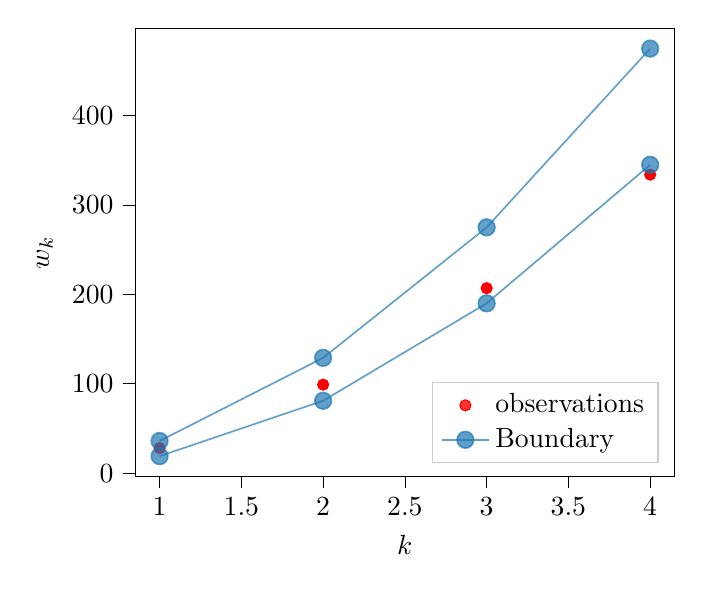
\begin{tikzpicture}

\definecolor{darkgray176}{RGB}{176,176,176}
\definecolor{lightgray204}{RGB}{204,204,204}
\definecolor{steelblue31119180}{RGB}{31,119,180}

\begin{axis}[
legend cell align={left},
legend style={
  fill opacity=0.8,
  draw opacity=1,
  text opacity=1,
  at={(0.97,0.03)},
  anchor=south east,
  draw=lightgray204
},
tick align=outside,
tick pos=left,
x grid style={darkgray176},
xlabel={\(\displaystyle k\)},
xmin=0.85, xmax=4.15,
xtick style={color=black},
y grid style={darkgray176},
ylabel={\(\displaystyle w_k\)},
ymin=-3.8, ymax=497.8,
ytick style={color=black}
]
\addplot [draw=red, fill=red, mark=*, only marks]
table{%
x  y
1 28
2 99
3 207
4 334
};
\addlegendentry{observations}
\addplot [semithick, steelblue31119180, opacity=0.7, mark=*, mark size=3, mark options={solid}]
table {%
1 19
2 81
3 190
4 345
};
\addlegendentry{Boundary}
\addplot [semithick, steelblue31119180, opacity=0.7, mark=*, mark size=3, mark options={solid}, forget plot]
table {%
1 36
2 129
3 275
4 475
};
\end{axis}

\end{tikzpicture}

\caption{Illustration of the boundary.\label{fig:gst}}
\end{center}
\end{figure}

\todoT{For now, the illustration is done using toy model, with gaussian of drift 0.7. Real agent would be better.}


\subsection{Speeding up permutation tests}
We use Monte-Carlo approximation, using random permutation instead of enumerating all the permutations.

\section{Multiple testing}
\subsection{Case of non-sequential permutation test}
When dealing with multiple testing, particular care must be taken so as not to decrease the error of the test. Suppose that we want to test $H_j$ versus $H_j'$ for $1\le j\le J$ using a test statistic $T_{n}^{(j)}$. Instead of the type I error considered in two-sample testing, we consider the family-wise error rate (FWE) which is defined as the probability of making at least one type I error:
$$\mathrm{FWE} = \P_{H_1,\dots,H_J}\left(\exists 1\le j\le J:\quad  \text{reject }H_j \right).$$

\paragraph{Bonferroni procedure:} a first approach is obtained by taking a threshold for $H_j$ vs $H_j'$ equal to a quantile of order $1-\alpha/J$ of the permutation distribution of $T_n^{(j)}$, this is the Bonferroni procedure and it can be very conservative.

\paragraph{Step-down procedure:} another approach proposed by \cite{Romano_2003} is to consider a step-down procedure defined as follows: for some $\textbf{K} \subset \{1,\dots,J\}$, denote
$$T_{n}^{(\textbf{K})}(\sigma)= \max\left(T_n^{(j)}(\sigma),\quad j \in \textbf{K}\right)$$

\begin{algorithm}[h]
\SetAlgoLined
\SetKwInput{KwParameter}{Parameters}
\KwParameter{$\alpha \in (0,1)$}
Initialize $\textbf{K}=\{1,\dots,J\}$\\
\While{$\textbf{K} \neq \emptyset$}{
Compute $\widehat{c}_{n}^{(\textbf{K})}(1-\alpha)$ the quantile of order $1-\alpha$ of the permutation law of $T_{n}^{(\textbf{K})}(\sigma)$:
$$\sum_{\sigma \in S_n} \1\{T_{n}^{(\textbf{K})}(\sigma) \ge  \widehat{c}_{n}^{(\textbf{K})}(1-\alpha)\} = \lfloor \alpha n! \rfloor .$$
\If{$T_{n}^{(\textbf{K})}(\mathrm{id}) \le \widehat{c}_{n}^{(\textbf{K})}(1-\alpha)$}{
Accept all the hypotheses $H_j, j\in \textbf{K}$ and break the loop.}
\Else{
Reject $H_{j_{\max}}$ where $j_{\max} =  \arg\max\left(T_n^{(j)}(\sigma),\quad j \in \textbf{K}\right)$.\\
Define $\textbf{K}=\textbf{K} \setminus \{j_{max}\}$
}
}
If the test was never rejected, return accept. Else return reject.
\caption{Multiple testing, non-sequential.}\label{alg:multiple_test_1}
\end{algorithm}
The Algorithm~\ref{alg:multiple_test_1} is consistent (i.e. $\mathrm{FWE}\le \alpha$) for the equality of distribution hypotheses.
\subsection{Sequential Step-Down method (Main algorithm)}
For some $\textbf{K} \subset \{1,\dots,J\}$, denote
$$T_{n,k}^{(\textbf{K})}(\sigma)= \max\left(\sum_{i=1}^kT_{n,i}^{(j)}(\sigma_i),\quad j \in \textbf{K}\right)$$
where
$$T_{n,i}^{(j)}(\sigma_i)= \sum_{l=1}^{n} e_{\sigma_i(l)+2ni}-\sum_{l=n+1}^{2n} e_{\sigma_i(l)+2ni} $$
is the mean difference on block $i$ after permutation by $\sigma_i$
\todoT{Add algorithm here}
% \begin{algorithm}[h]
% \SetAlgoLined
% \SetKwInput{KwParameter}{Parameters}
% \KwParameter{Agents $A_1,A_2$, environment $\mathcal{E}$, number of blocks $K \in \N^*$, size of a block $n$, level of the test $\alpha\in (0,1)$.}
% Define $2nK$ different seeds $s_{1,1},\dots,s_{1,n},s_{2,1},\dots,s_{2,n}$.\\
% \For{$k=1,\dots,K$}{
% \For{$i=1,2$}{
% Train agent $A_i$ on environment $\mathcal{E}$ with the seeds $s_{i,kn},\dots,s_{i,(k+1)n}$.\\
% Collect evaluations $e_{kn}(A_i),\dots,e_{(k+1)n}(A_i)$.\\
% Compute $S_t(A_i)=\frac{1}{nk}\sum_{j=1}^{nk}e_{j}(A_i)$.\\
% }
% Compute $T$.\\
% \If{$|S_t(A_1)-S_t(A_2)| \ge B_k$}{
% Reject the equality of the agents' evaluation, break the loop and returns the answer
% }
% \Else{
% If $k=K$ then accept the equality of the agents' evaluation, otherwise continue.
% }
% }
% If the test was never rejected, return accept. Else return reject.
% \caption{Adastop for multiple agents}\label{alg:adastop_2}
% \end{algorithm}
\section{Asymptotic study}
\subsection{Case of a non-sequential permutation test}

Foor a sample $Z_1^n=(Z_1,\dots,Z_n)$, denote $\sigma Z_1^n$ the permuted sample using the permutation $\sigma$: $\sigma Z_1^n=(Z_{\sigma(1)},\dots,Z_{\sigma(n)})$.\\
For $T_n$ the difference of empirical mean, we have the following property.

\begin{Proposition}\label{prop:asym_perm_test}
Let $T_n(Z_1,\dots,Z_{2n})=\frac{1}{\sqrt{n}}\sum_{i=1}^n Z_i -\frac{1}{n}\sum_{i=n+1}^{2n} Z_i$.

Suppose $X_1,\dots,X_n$ are i.i.d from $P$ and $Y_1,\dots,Y_n$ are i.i.d from $Q$ and both $P$ and $Q$ has finite variance. Denote $Z_1,\dots,Z_{2n}=X_1,\dots,X_n, Y_1,\dots,Y_n$ the concatenation of the two samples. Then, we have
$$\sup_{t}\left|\frac{1}{n!}\sum_{\sigma \in S_n} \1\{T_n(\sigma Z_{1}^{2n}) \le t\}- \Phi\left(t/\tau(P,Q) \right)\right|\xrightarrow[n \to \infty]{P} 0$$
where $\tau(P,Q)^2=\sigma_P^2+\sigma_Q^2+\frac{(\mu_P- \mu_Q)^2}{2} $.
\end{Proposition}
Remark: this proposition can be extended to other $T_n$ statistics using Theorem 2.1 in \cite{Chung_2013} or Theorem 15.2.5 of \cite{lehmann2005testing}.
%\todoT{Maybe I could do an edgeworth expansion to show that the convergence is with speed $1/n$ (under $H_0$ ?) because of the symmetry of $T$. Using \cite{Romano_1990} and \cite[Theorem 7]{Petrov_1975}. The expansion could be used to derive an approximation of the power that could be used to set K beforehand.}
%\todoT{Another possible interesting result would be to show how many random permutations we need to estimate the true permutation distribution. Concentration inequalities could be used here.}

Using Proposition~\ref{prop:asym_perm_test}, we have that the empirical quantile defined by
$$Q_{1-\alpha}(T_n) = \inf\left\{t \in \R:\quad \frac{1}{n!}\sum_{\sigma \in S_n} \1\{T_n(\sigma Z_{1}^{2n}) \le t\} \ge 1-\alpha\right\} $$
converges to the quantiles of a Gaussian with variance $\tau^2$
$$Q_{1-\alpha}(T_n)\xrightarrow[n \to \infty]{P} \tau(P,Q)\Phi^{-1}(1-\alpha) $$

 Hence, if $\mu_P = \mu_Q$ is true, in which case $T_n$ converges in distribution to $T_\infty\sim \mathcal{N}(0,\sigma_P^2+\sigma_Q^2 )$ and then
$$\P\left( T_n \ge Q_{1-\alpha}(T_n)\right) \xrightarrow[n \to \infty]{} \P(T_\infty\ge \tau(P,Q)\Phi^{-1}(1-\alpha)) \ge  1-\Phi\left(\tau(P,Q)\frac{\Phi^{-1}(1-\alpha)}{\sigma_P^2+\sigma_Q^2 } \right)=\alpha  $$

On the other hand, if $\mu_P > \mu_Q$, then $T_n \simeq \mathcal{N}(\sqrt{n}(\mu_P-\mu_Q),\sigma_P^2+\sigma_Q^2 ) $

\begin{align*}
\P\left( T_n \ge Q_{1-\alpha}(T_n)\right)&\simeq  1-\Phi\left(\tau(P,Q)\frac{\Phi^{-1}(1-\alpha)}{\sigma_P^2+\sigma_Q^2 }-  \sqrt{n}\frac{\mu_P-\mu_Q}{\sqrt{\sigma_P^2+\sigma_Q^2}} \right)  \\
&\simeq  1-\Phi\left(\Phi^{-1}(1-\alpha)\left(1+\frac{(\mu_P-\mu_Q)^2}{\sigma_P^2+\sigma_Q^2 }\right)-  \sqrt{n}\frac{\mu_P-\mu_Q}{\sqrt{\sigma_P^2+\sigma_Q^2}} \right)
\end{align*}
For a given drift $\mu_P-\mu_Q$, we can solve for $n$ to get a sample size required in order to converge to a given power.

Example: suppose we want to detect a drift $\mu_P-\mu_Q=\sqrt{\sigma_P^2+\sigma_Q^2}$ in with probability $0.9$. Then we solve $1-\Phi\left(\Phi^{-1}(1-\alpha)\left(1+\frac{(\mu_P-\mu_Q)^2}{\sigma_P^2+\sigma_Q^2 }\right)-  \sqrt{n}\frac{\mu_P-\mu_Q}{\sqrt{\sigma_P^2+\sigma_Q^2}} \right) = 0.9$ and get that $n$ must be larger than $21$.

\subsection{Permutation Group Sequential tests}

Denote $S_{i}^{i+j}=(S_i, S_{i+1},\dots, S_{i+j})$ and let $T_n(S_1^n)=T(S_1,\dots,S_{2n})=\frac{1}{\sqrt{n}}\sum_{i=1}^n S_i -\frac{1}{n}\sum_{i=n+1}^{2n} S_i$. Denote by
$$\widehat{R}_{n,k}(t)=\frac{1}{n!}\sum_{\sigma \in S_{2n}} \1\{\sqrt{n}T_n(\sigma S_{2nk}^{2n(k+1)}) \le t\} $$
the randomization distribution of $T_n$ where for any permutation $\sigma \in S_n$,
$$\sigma S_{2nk}^{2n(k+1)}=(S_{\sigma(2nk)},S_{\sigma(2nk+1)},\dots,S_{\sigma(2n(k+1))})$$
is the sample permuted using $ \sigma$.


% We have
% \begin{align*}
% \prod_{k=1}^K \widehat{R}_{n,k}(t_k) &=\frac{1}{(n!)^K}\sum_{\sigma_1,\dots,\sigma_K \in S_{2n}} \prod_{k=1}^K \1\{\sqrt{n}T_n(\sigma S_{2nk}^{2n(k+1)}) \le t_k\} \\
% &=\frac{1}{(n!)^K}\sum_{\sigma_1,\dots,\sigma_K \in S_{2n}}  \1\{ \forall 1\le k\le K, \quad \sqrt{n} T_n(\sigma S_{2nk}^{2n(k+1)}) \le t_k\}
% \end{align*}
% We have
% \begin{align*}
% \sup_{t}&\left|\prod_{k=1}^K \widehat{R}_{n,k}(t_k) - \prod_{k=1}^K \Phi\left( \frac{t_k}{\tau(P,Q)}\right) \right| \\
% &= \sup_t \left| \widehat{R}_{n,K}(t_K)\left(\prod_{k=1}^{K-1} \widehat{R}_{n,k}(t_k) - \prod_{k=1}^{K-1}\Phi\left( \frac{t_k}{\tau(P,Q)}\right)\right) + (\widehat{R}_{n,K}(t_K)-\Phi(t_K/\tau(P,Q))) \prod_{k=1}^{K-1} \Phi(t_k/\tau(P,Q))\right|\\
% &\le \sup_t \left| \widehat{R}_{n,K}(t_K)\left(\prod_{k=1}^{K-1} \widehat{R}_{n,k}(t_k) -\prod_{k=1}^{K-1} \Phi\left( \frac{t_k}{\tau(P,Q)}\right)\right)\right| + \sup_t\left|(\widehat{R}_{n,K}(t_K)-\Phi(t_K/\tau(P,Q))) \prod_{k=1}^{K-1}\Phi(t_k/\tau(P,Q)) \right|\\
% &\le \sup_t \left|\prod_{k=1}^{K-1} \widehat{R}_{n,k}(t_k) - \prod_{k=1}^{K-1}\Phi\left( \frac{t_k}{\tau(P,Q)}\right)\right| + \sup_t\left|\widehat{R}_{n,K}(t_K)-\Phi(t_K/\tau(P,Q)) \right|
% \end{align*}
% Hence, reasoning by induction, we have from Proposition~\ref{prop:asym_perm_test}
% $$\sup_{t}\left|\prod_{k=1}^K \widehat{R}_{n,k}(t_k) - \prod_{k=1}^{K}\Phi\left( \frac{t_k}{\tau(P,Q)}\right) \right|\xrightarrow[n \to \infty]{P} 0$$

\textbf{Convergence of the boundary}

Notation:
$$T_{n,k}(\sigma)=T_n\left(\sigma S_{2nk+1}^{2n(k+1)}\right) $$
is the difference of the means on the $k^{th}$ bloc when the block have been permuted using $\sigma$.

Remark that on the first step, because the conditional distribution of $T_n(\sigma S_1^{2n})$ knowing $S_1^{2n}$ is symmetric, there is no need to compute the lower boundary and the decision can be made solely by testing $|T_n(S_1^{2n})|\ge B_1$ for some $B_1$. The same reasoning can be used for the remaining steps.

The boundaries are the minimal values of $B_1,\dots, B_K$ such that

$$\P_{\sigma_1}(|T_{n,1}(\sigma_1)|\ge B_1) = q_1 \le \alpha\left(\frac{1}{K}\right) $$

$$\P_{\sigma_1^2}\left( \frac{1}{2}|T_{n,2}(\sigma_2)+T_{n,1}(\sigma_1)|\ge  B_2\sqrt{n},\quad  |T_{n,1}(\sigma_1)|\le  B_1\sqrt{n}  \right)+q_1 = q_2 \le\alpha\left(\frac{2}{K}\right) $$
More generally, for any $2\le k\le K$,
\begin{equation}\label{eq:def_Bk}
\P_{\sigma_1^k}\left(\left|\frac{1}{k}\sum_{j=0}^k T_{n,j}(\sigma_j)\right|\ge B_{k}, \quad \forall i < k,\,  n\left|\frac{1}{i}\sum_{j=0}^i T_{n,j}\left(\sigma_j\right)\right|\le  B_i\right)+\sum_{j=1}^{k-1}q_j  = q_k \le\alpha\left(\frac{k}{K}\right).
\end{equation}
Remark that $B_k$ is deterministic conditionally on the values of $S_1,\dots,S_{2nk}$. Hence it is deterministic with respect to the random permutation $\sigma$, but it still depends on $n$ and the values of $S_i$.

\begin{Theorem}\label{th:conv_boundary}
We have that for any $1\le k\le K$, $B_k\xrightarrow[n \to \infty]{}b_k$ where the real numbers $b_k$ are defined as follows. Let $W_1,\dots, W_K$ be i.i.d random variable with law $\mathcal{N}(0,1)$, then $b_1$ is the solution of the following equation:
$$ \P\left(\left|W_1 \right|\ge \frac{b_1}{\tau(P,Q)}  \right)=\alpha\left( \frac{1}{K} \right),$$
and for any $1<k\le K$, $b_k$ is solution of
\begin{equation*}
\P\left( \left|\frac{1}{k}\sum_{j=1}^k W_j\right| > \frac{b_l}{\tau(P,Q)}, \quad \forall j<k,\, \left|\frac{1}{j}\sum_{i=1}^j W_i\right| \le \frac{b_j}{\tau(P,Q)} \right)=\alpha\left(\frac{k}{K} \right) - \alpha\left( \frac{k-1}{K}\right).
\end{equation*}

\end{Theorem}
In short, Theorem~\ref{th:conv_boundary} tells us that asymptotically, the group sequential test behaves like a sequential test on Gaussians in which the boundary is set to spend the level $\alpha$ exactly as predicted by the level-spending function. There are several consequences of this theorem.
\todoT{Show this properly with lemmas and proving everything}
\begin{itemize}
 \item Asymptotically, the test $H_0:\mu_X = \mu_Y$ vs $H_1:\mu_X \neq \mu_Y$ has level $\alpha$ because under $H_0$, $\tau(P,Q)^2=\sigma_P^2+\sigma_Q^2$ and $T_n(\mathrm{id} S_1^{2n})=\frac{1}{\sqrt{n}}\left(\sum_{i=1}^n S_i - \sum_{i=n+1}^{2n} S_i\right)$ converges to $\mathcal{N}(0,\sigma_X^2+\sigma_Y^2)$. Hence the boundary correspond to the appropriate law.
 \item Under $H_1:\mu_P \neq \mu_Q$, we have an expression of the asymptotic boundary. On the other hand, we also have that
$$T_n(\mathrm{id}S_1^{2n}) =\frac{1}{\sqrt{n}}\left(\sum_{i=1}^n S_i - \sum_{i=n+1}^{2n} S_i\right) = \frac{1}{\sqrt{n}}\left(\sum_{i=1}^n (S_i-\mu_X) - \sum_{i=n+1}^{2n} (S_i-\mu_Y)   + n (\mu_X-\mu_Y)\right)$$
Hence, because the convergence in the CLT is uniform, we have
$$\P\left( T_n(\mathrm{id}S_1^{2n}) \le B_1\right) = \Phi\left(\frac{B_1-\sqrt{n}(\mu_X-\mu_Y)}{\sqrt{\sigma_X^2+\sigma_Y^2}}\right) + o_P(1).$$
Then, by Theorem~\ref{th:conv_boundary},
$$\P\left( T_n(\mathrm{id}S_1^{2n}) \le B_1\right) = \Phi\left(\frac{b_1+o_P(1)-\sqrt{n}(\mu_X-\mu_Y)}{\sqrt{\sigma_X^2+\sigma_Y^2}}\right) + o_P(1) =\Phi\left(\frac{b_1-\sqrt{n}(\mu_X-\mu_Y)}{\sqrt{\sigma_X^2+\sigma_Y^2}}\right) + o_P(1)$$
Then, repeating the same reasoning on $\P\left( T_n(\mathrm{id}S_1^{2n}) \ge - B_1\right)$, we obtain, the probability to reject at the first interim given by
$$\P\left( |T_n(\mathrm{id}S_1^{2n})| > B_1\right) = \P\left( \left|W_1\sqrt{\sigma_X^2+\sigma_Y^2}-\sqrt{n}(\mu_X-\mu_Y)\right|\ge b_1\right) + o_P(1).$$
Proceeding similarly, we have that there exists $W_1,\dots,W_K$ i.i.d. $\mathcal{N}(0,1)$ random variables such that
$$\P\left( \exists k \le K:\, \left|\frac{1}{k}\sum_{j=1}^k T_{n,j}(\mathrm{id})\right| > B_k\right) =\P\left( \exists k \le K:\, \left|\frac{\sqrt{\sigma_X^2+\sigma_Y^2}}{k}\sum_{j=1}^kW_j + \sqrt{n}(\mu_X-\mu_Y)\right| > b_k\right) + o_P(1).$$
This approximation of the power can be computed approximately using Monte-Carlo methods, using gaussian concentration inequality to know how many Monte-Carlo iteration are necessary to approximate the power.
% One way to bound this is to state that
% \begin{align*}
% \P&\left( \exists k \le K:\, \left| \frac{\sqrt{\sigma_X^2+\sigma_Y^2}}{k}\sum_{j=1}^kW_j + \sqrt{n}(\mu_X-\mu_Y)\right| > b_k\right)\\
% & \ge  \P\left( \exists k \le K:\,\left| \frac{\sqrt{\sigma_X^2+\sigma_Y^2}}{k}\sum_{j=1}^kW_j \right|  < -b_k+\sqrt{n}|\mu_X-\mu_Y|\right)\\
% & \ge  \P\left(  \frac{\sqrt{\sigma_X^2+\sigma_Y^2}}{K}\left|\sum_{j=1}^KW_j \right| +b_K < \sqrt{n}|\mu_X-\mu_Y|\right)\\
% \end{align*}

\end{itemize}
\section{Proof of Theorem~\ref{th:conv_boundary}}
\paragraph{Convergence of $B_1$}
$$B_1 = \min \left\{ b>0 : \P_\sigma(|T_{n,1}(\sigma_1)|\ge b) \le \alpha\left(\frac{1}{K}\right)\right\} $$
This implies
$$\P_\sigma(|T_{n,1}(\sigma_1)|\le B_1) = \widehat{R}_{n,1}\left(B_1\right)-\widehat{R}_{n,1}\left(-B_1\right) \ge 1-\alpha\left( \frac{1}{K} \right) $$
and for any $b < B_1$, we have
$$\P_\sigma(|T_{n,1}(\sigma_1)|\le b)=\widehat{R}_{n,1}\left(b\right)-\widehat{R}_{n,1}\left(b\right) < 1- \alpha\left( \frac{1}{K} \right) $$
Then,
\begin{align*}
\Phi&\left( \frac{B_1}{\tau(P,Q)}\right)-\Phi\left(-\frac{B_1}{\tau(P,Q)}\right)\\
 &\ge \widehat{R}_{n,1}\left(B_1\right)-\widehat{R}_{n,1}\left(-B_1\right)-\left|\Phi\left( \frac{B_1}{\tau(P,Q)}\right) -\widehat{R}_{n,1}\left(B_1\right) \right|-\left|\Phi\left( -\frac{B_1}{\tau(P,Q)}\right) -\widehat{R}_{n,1}\left(-B_1\right) \right| \\
&\ge1- \alpha\left( \frac{1}{K} \right)- 2\sup_{t}\left|\Phi\left( \frac{t}{\tau(P,Q)}\right) -\widehat{R}_{n,1}\left(t\right) \right|
\end{align*}
Hence, by taking $n$ to infinity, we have
$$\liminf_{n \to \infty} \Phi\left( \frac{B_1}{\tau(P,Q)}\right)-\Phi\left(-\frac{B_1}{\tau(P,Q)}\right) \ge 1-\alpha\left( \frac{1}{K} \right).$$
and for any $\varepsilon>0$, we have
$$\limsup_{n \to \infty} \Phi\left( \frac{B_1+\varepsilon}{\tau(P,Q)}\right)-\Phi\left( -\frac{B_1+\varepsilon}{\tau(P,Q)}\right) < 1- \alpha\left( \frac{1}{K} \right).$$
\todoT{Maybe explain this a bit more}
By continuity of $\Phi$, this implies that $B_1$ converges almost surely and its limit is such that
$$\Phi\left( \frac{\lim_{n \to \infty}B_1}{\tau(P,Q)}\right)-\Phi\left( -\frac{\lim_{n \to \infty}B_1}{\tau(P,Q)}\right)= 1-\alpha\left( \frac{1}{K} \right).$$
\todoT{There is a switch of two limits here, check it}
Or said differently, let $W\sim \mathcal{N}(0,1)$, the we have the almost sure convergence $\lim_{n \to \infty}B_1 = b_1$ where $b_1$ is the real number defined by
$$ \P\left(\left|W \right|\ge \frac{b_1}{\tau(P,Q)}  \right)=\alpha\left( \frac{1}{K} \right).$$

\paragraph{Convergence of $B_k$ for $k>1$.}

We proceed by induction. Suppose that for all $l <k$, $B_l$ converges to $b_l$ defined by

\begin{equation}\label{eq:induction_hyp}
\P\left( \left|\frac{1}{l}\sum_{j=1}^l W_j\right| > \frac{b_l}{\tau(P,Q)}, \quad \forall j<l,\, \left|\frac{1}{j}\sum_{i=1}^j W_i\right| \le \frac{b_j}{\tau(P,Q)} \right)=\alpha\left(\frac{l}{K} \right) - \alpha\left( \frac{l-1}{K}\right).
\end{equation}

We have
$$B_k = \min \left\{ b>0 : \P_{\sigma_1^k}\left(\left|\frac{1}{k}\sum_{j=0}^k T_{n,j}\left(\sigma_j\right)\right|\ge b, \quad \forall j < k,\,  \left|\frac{1}{j}\sum_{i=0}^j T_{n,i}\left(\sigma_i\right)\right|\le  B_j  \right)+\sum_{i=1}^{k-1}q_i \le\alpha\left(\frac{k}{K}\right)\right\}.$$

By the recurrence hypothesis, we have $q_i \xrightarrow[n \to \infty]{}\alpha\left( \frac{i}{K} \right)-\alpha\left( \frac{i-1}{K} \right)$ and $q_1\xrightarrow[n \to \infty]{}\alpha\left( \frac{1}{K} \right)$.

Let $W_1,\dots,W_k$ be i.i.d $\mathcal{N}(0,1)$ random variables. Denote
$$\Psi_k(b) = \P\left( \frac{1}{k}\sum_{j=1}^k W_j \le \frac{b}{\tau(P,Q)}, \quad \forall j<k,\, \left|\frac{1}{j}\sum_{i=1}^j W_i\right| \le \frac{b_j}{\tau(P,Q)} \right) $$
We will need the following lemma, proved in Section~\ref{sec:proof_lem_conv}.
\begin{Lemma}\label{lem:convergence_conditional}
Suppose Equation~\eqref{eq:induction_hyp} is true. Then,
$$\sup_{b}\left|\P_{\sigma_1^{k}}\left(\frac{1}{k}\sum_{j=1}^k T_{n,j}\left(\sigma_j\right)\le b \sqrt{n}, \quad \forall j < k,\,  \left|\frac{1}{j}\sum_{i=1}^j T_{n,i}\left(\sigma_i\right)\right|\le  B_j\sqrt{n} \right)-\Psi_k(b) \right|\xrightarrow[n \to \infty]{}0$$
\end{Lemma}
We have, conditionally on $B_k$,
\begin{align*}
\Psi_k(B_k)-\Psi_k(-B_k)\ge&  \P_{\sigma_1^{k}}\left(\left|\frac{1}{k}\sum_{j=1}^k T_{n,j}\left(\sigma_j\right)\right|\le B_k \sqrt{n}, \quad \forall j < k,\,  \left|\frac{1}{j}\sum_{i=1}^j T_{n,i}\left(\sigma_i\right)\right|\le  B_j \right)\\
&+ 2 \sup_{b}\left|\P_{\sigma_1^{k}}\left(\frac{1}{k}\sum_{j=1}^k T_{n,j}\left(\sigma_j\right)\le b , \quad \forall j < k,\,  \left|\frac{1}{j}\sum_{i=1}^j T_{n,i}\left(\sigma_i\right)\right|\le  B_j \right)-\Psi_k(b) \right|\\
&\ge 1-\left(\alpha\left( \frac{k}{K}\right)-\sum_{i=1}^{k-1}q_i\right) \\
&+ 2 \sup_{b}\left|\P_{\sigma_1^{k}}\left(\frac{1}{k}\sum_{j=1}^k T_{n,j}\left(\sigma_j\right)\le b , \quad \forall j < k,\,  \left|\frac{1}{j}\sum_{i=1}^j T_{n,i}\left(\sigma_i\right)\right|\le  B_j \right)-\Psi_k(b) \right|
\end{align*}
We use Lemma~\ref{lem:convergence_conditional} and the convergence of the $q_i$'s to conclude that
$$\liminf_{n \to \infty}\Psi_k(B_k)-\Psi_k(-B_k) \ge 1-\left(\alpha\left( \frac{k}{K}\right)-\alpha\left( \frac{k-1}{K}\right)\right).$$
And similarly to the case $k=1$, we also have for any $\varepsilon>0$,
$$\limsup_{n \to \infty}\Psi_k(B_k+\varepsilon)-\Psi_k(-B_k-\varepsilon) \le  1-\left(\alpha\left( \frac{k}{K}\right)-\alpha\left( \frac{k-1}{K}\right)\right).$$
and by continuity of $\Psi_k$ we conclude that $B_k$ converges almost surely to $b_k$.
\todoT{Check continuity of $\Psi_k$}
\section{Proof of Lemmas}
\subsection{Proof of Lemma~\ref{lem:convergence_conditional}}\label{sec:proof_lem_conv}
\begin{align*}
\P_\sigma&\left(\frac{1}{k}\sum_{j=1}^k T_{n,j}\left(\sigma_j\right)\le b , \quad \forall j < k,\,  \left|\frac{1}{j}\sum_{i=1}^j T_{n,i}\left(\sigma_i\right)\right|\le  B_j  \right)\\
&= \E_{\sigma_1^{k-1}} \left[ \P_{\sigma_k}\left(\frac{1}{k}\sum_{j=0}^k T_{n,j}\left(\sigma_j\right)\le b \right)\1\left\{ \forall j < k,\,  \left|\frac{1}{j}\sum_{i=1}^j T_{n,i}\left(\sigma_j\right)\right|\le  B_j\right\}\right]
\end{align*}
Now, conditionally on the permutations $\sigma_1^{k-1}=\sigma_1,\dots,\sigma_{k-1}$, we have
\begin{align*}
\P_{\sigma_k}\left(\frac{1}{k}\sum_{j=0}^k T_{n,j}\left(\sigma_j\right)\le b \sqrt{n}\right) &= \P_{\sigma_k}\left( \frac{1}{k}T_{n,k}\left(\sigma_k\right)\le b -\frac{1}{k}\sum_{j=1}^{k-1}T_{n,j}\left(\sigma_j\right) \right)\\
&= \widehat{R}_{n,k}\left(bk-n\sum_{j=1}^{k-1}T_{n,j}\left(\sigma_j\right)\right)
\end{align*}
We have, because the convergence is uniform,
\begin{align*}
&\hspace{-3em}\left|\E_{\sigma_1^{k-1}} \left[ \P_{\sigma_k}\left(\frac{1}{k}\sum_{j=0}^k T_{n,j}\left(\sigma_j\right)\le b\right)\1\left\{ \forall j < k,\,  \left|\frac{1}{j}\sum_{i=1}^j T_{n,i}\left(\sigma_j\right)\right|\le  B_j\right\}\right]\right.\\
&\hspace{-1em}\left.- \E_{\sigma_1^{k-1}} \left[ \Phi\left( bk - \sum_{j=1}^{k-1}T_{n,j}(\sigma_j) \right)\1\left\{ \forall j < k,\,  \left|\frac{1}{j}\sum_{i=1}^j T_{n,i}\left(\sigma_j\right)\right|\le  B_j\right\}\right] \right|\\
&\le \E_{\sigma_1^{k-1}} \left[ \left|\P_{\sigma_k}\left(\frac{1}{k}\sum_{j=0}^k T_{n,j}\left(\sigma_j\right)\le b \right)- \Phi\left( \frac{bk - \sum_{j=1}^{k-1}T_{n,j}(\sigma_j) }{\tau(P,Q)}\right)\right|\right]\\
&= \E_{\sigma_1^{k-1}} \left[ \left|\P_{\sigma_k}\left( T_{n,k}\left(\sigma_k\right)\le bk - \sum_{j=1}^{k-1} T_{n,j}(\sigma_j) \right)- \Phi\left( \frac{bk - \sum_{j=1}^{k-1}T_{n,j}(\sigma_j) }{\tau(P,Q)}\right)\right|\right]\\
&\le \sup_t \left|\widehat{R}_n(t)-\Phi\left( \frac{t}{\tau(P,Q)}\right)\right|  \xrightarrow[n \to \infty]{}0
\end{align*}
Finally, use that by hypothesis, $B_j \to b_j$ and $T_{n,j} \to W_j$ to conclude that the lemma is true by dominated convergence.
\todoT{Maybe explain this further}
\newpage
\section{Simulation study}
\todoT{Misspecification study of Gaussian GST on uniform and maybe on multi-modal distributions}
\todoT{Comparison of GST algorithms on gaussian Data.}
\section{Experimental results}
\todoT{Apply to some classical algorithms on classical environments. Maybe also try to
replicate adaptively the results of the NIPS article : do we also stop around 20 iterations when comparing two agents on an Atari environment?}
\todoT{Compare with article https://arxiv.org/pdf/1806.08295.pdf on environments that are simpler than Atari. Maybe show that depending on the environment the number of seeds needed can vary a lot.}
% \section{Other possible algorithms}
% \begin{algorithm}[h]
% \SetAlgoLined
% \SetKwInput{KwParameter}{Parameters}
% \KwParameter{Evaluations $e_1(A_i),\dots,e_t(A_i)$ for $i \in \{1,2\}$, level of the test $\alpha$, number of blocks $K$, number of permutations $B$.}
% Compute $t_0=S_t(A_1)-S_t(A_2)$.\\
% Define $Z_1,\dots,Z_{2t}$ with
% $$Z_i = \begin{cases}e_i(A_1) & \text{ if }1\le i\le t\\ e_{i-t}(A) & \text{ if }t+1\le i\le 2t \end{cases} $$
% \For{$b=1,\dots,B$}{
% Draw a permutation $\sigma$ uniformly at random in $\mathcal{S}_{2t}$.\\
% Compute
% $$t_b = \frac{1}{t}\sum_{i=1}^t Z_{\sigma(i)}-\frac{1}{t}\sum_{i=t+1}^{2t} Z_{\sigma(i)}$$
% }
% Let $q_1$ be the empirical quantile of level $\frac{\alpha}{2K}$ of $t_1,\dots,t_B$ and $q_2$ the empirical quantile of level $1-\frac{\alpha}{2K}$.\\
% If $t_0\le q_1$ or $t_0 \ge q_2$  then reject $H_0$. Else, do not reject $H_0$.
% \caption{Step $t$ of Union Bound Permutation GST.}\label{alg:gst}
% \end{algorithm}

\bibliographystyle{plain}
\bibliography{Adastop}
\end{document}
